\documentclass[spanish,draft,12pt,headsepline,footsepline,paper=letter]{scrreprt}
\pagestyle{headings}

\usepackage[utf8]{inputenc}
\usepackage[T1]{fontenc}
\def\spanishoptions{es-noquoting,es-nolists,mexico-com}
\usepackage[spanish]{babel}

\usepackage[final]{graphicx}
\DeclareGraphicsExtensions{.pdf,.png,.jpg}
\graphicspath{{media/}}
\usepackage{rotating}

\usepackage{scrhack}

\usepackage{natbib}
\usepackage{amsmath,amssymb, bm}
\usepackage{enumerate}
\usepackage{ragged2e}
\usepackage{nameref}

\usepackage{setspace}
\onehalfspacing
\frenchspacing
\recalctypearea

\begin{document}

\title{Protocolo de Investigación: Programación de horarios educacionales}
\author{Héctor Arciga}
\date{\today}

\maketitle

\section*{Introducción}
Esta propuesta de investigación atañe la programación de horarios educacionales. Presenta los objetivos de la investigación, su justificación y las preguntas de investigación. También incluye una reseña general de la literatura pertinente y finaliza delineando un diseño de la investigación así como su índice y plan de trabajo tentativos.

\section*{Objetivos de la investigación}
Mucho se ha discutido acerca de cómo mejorar el desempeño de las instituciones educativas, predominan cavilaciones que sugieren la inversión en infraestructura; la capacitación continua de los docentes; el aprovisionamiento gratuito de útiles escolares, uniformes, alimentos; la  inclusión de nuevas tecnologías informáticas en el proceso de enseñanza; mejoras en las condiciones laborales del magisterio; entre muchas otras. 

A pesar de la complejidad del sistema educativo, toda institución cuenta con los mismos elementos básicos: alumnos, profesores, aulas, clases, asignaturas y lecciones. La conformación de estos en un programa educacional establece dinámicas de vasto alcance trastocando aspectos operacionales en ámbitos pedagógicos, financieros, laborales, regulatorios y sociales.

La pregunta estratégica que orienta esta investigación es: 

«¿Cómo se debe elaborar un horario escolar para incidir en el desempeño de una institución educacional persiguiendo objetivos específicos?»

\subsection*{Objetivo general}

El fin primordial de la investigación es determinar cómo puede el gestor escolar incidir en las métricas de desempeño relevantes, a través de la conformación de los horarios escolares.

\subsection*{Objetivos específicos}
Para poder cumplir con esta finalidad, los siguientes objetivos son considerados: \begin{enumerate}[1]
\setlength{\itemsep}{0cm}%
\setlength{\parskip}{0cm}%
\item La exposición clara y concisa de los elementos de la programación
\item La revisión bibliográfica del marco teórico de la programación
\item El detallado de la problemática de la programación en el ámbito educacional
\item El análisis de las métricas de desempeño educacional relevantes para los gestores escolares.
\item Los posibles alcances de un programa educacional en los ámbitos pedagógicos, financieros, laborales, regulatorios y sociales.
\end{enumerate}

\section*{Justificación}

\textit{Opción 1:}

En la actualidad la formación del individuo ha sido arrebatada por el Estado bajo falsas pretensiones. Es mi convicción que la esencia de una sociedad la define el actuar de sus individuos y es derecho divino de la familia transmitir sus propios valores, creencias e historia a sus futuras generaciones. El sistema educativo moderno apuesta por la transformación social, a conveniencia de los intereses de terceros, erosionando día a día la cultura propia de la comunidad. La institucionalización de la educación tiene un impacto profundo en el tejido social; su rol en la transformación social es cada vez más aparente conforme avanza la globalización, estandarizando los procesos educacionales. Es necesario crear alternativas para quienes deseamos que la educación sea en servicio del individuo, su familia y comunidad; para ello es fundamental contar con herramientas que permitan experimentar ampliamente con la estructura y procesos de la institución educativa, facilitando a la vez su evaluación, de acuerdo a los intereses propios de la institución. 

\textit{Opción 2:}

El desarrollo de los horarios escolares busca hacer un mejor uso de los recursos con los que cuenta la institución. La infraestructura de la institución se utiliza adecuadamente, respetando capacidades de utilización, tiempos de mantenimiento y aseo, evitando conflictos de uso. La planta docente se beneficia al tomar en cuenta los intereses del profesor respecto a sus preferencias de trabajo. El alumno obtiene un horario escolar que le permite compactar su tiempo de estudio, respetando tiempos de descanso y evitando conflictos entre sus cursos.

De igual manera, al crear un ambiente de trabajo en donde la planta docente, el alumnado y los recursos de la institución son estudiados y tomados en cuenta para su calendarización se pretende elevar la calidad educativa impartida en dicha institución.

\section*{Preguntas de investigación}

Las preguntas de investigación que se proponen son:

\begin{enumerate}[1]
\setlength{\itemsep}{0cm}%
\setlength{\parskip}{0cm}%
\item ¿Cuáles son los alcances de un horario escolar en los procesos educativos de una institución?
\item ¿Qué objetivos son los que persigue el gestor escolar al elaborar un horario?
\item ¿Qué elementos participan en la elaboración de un horario escolar?
\item ¿Cuáles son las métricas de desempeño relevantes en el ámbito educacional?
\item ¿De qué manera el horario escolar puede incidir en tales métricas de desempeño?
\item ¿Cómo se soluciona de manera sistemática un problema de programación?
\end{enumerate}

\section*{Hipótesis}

La aplicación de métodos formales de programación facilitan la elaboración de horarios escolares de acuerdo a objetivos planteados por el gestor escolar.

\section*{Marco teórico}

\subsection*{Reseña de los principales autores en el área}

PENDIENTE

\subsection*{Marco conceptual}

Para \citet[p.~5]{TKindt2002} los problemas de programación se encuentran en todo tipo de sistemas puesto que es necesaria para la organización y/o distribución del trabajo entre múltiples entidades. En cada libro pertinente de la literatura se presenta una definición así como sus componentes principales. Una de éstas es la enunciada por \citet{carlier1988problemes}: 
\begin{quotation}
La programación es predecir el procesamiento de un trabajo al asignar recursos a tareas y fijar sus tiempos de inicio\ldots Los diferentes componentes de un problema de programación son las tareas, sus restricciones potenciales, los recursos y la función objetivo\ldots Las tareas deben ser programadas para optimar un objetivo específico\ldots Por supuesto, frecuentemente será más realista en la práctica considerar múltiples criterios (como está citado en \citealp[p.~6]{TKindt2002}) 
\end{quotation}

Otra definición es la hecha por \citet[p.~1]{Pinedo1995}: «La programación es un proceso de toma de decisión\ldots  Se encarga de la asignación de recursos a tareas durante periodos y cuya meta es la optimación de uno o más objetivos.»

El objetivo de la programación es:

\begin{quotation}
  solucionar problemas prácticos relacionados a la asignación, sujeta a restricciones, de recursos a objetos siendo colocados en el espacio-tiempo, haciendo uso o desarrollando herramientas apropiadas. Los problemas con frecuencia buscarán la satisfacción de ciertos objetivos.
\end{quotation}


El problema de la programación de horarios educacionales\index{horarios!educacionales} se clasifica en tres clases principalmente:
calendarización de clases\index{horarios!de clases} (\textit{school timetabling}),
calendarización de cursos\index{calendarización!de cursos} (\textit{course timetabling}) y
calendarización de exámenes\index{calendarización!de exámenes} (\textit{examination timetabling}) \citep[p.~88]{schaerf99a-survey-of-automated}.

Todos tienen en común las características básicas del problema general de programación de horarios\index{horarios!problema general} pero pueden presentar diferencias significativas entre ellos. Cada problema cuenta con su propias restricciones\index{restricción}, requerimientos\index{requerimiento} y reglas\index{regla}. Son agrupados por su ámbito de aplicación en horarios en escuelas\index{horarios!en escuelas} y horarios en universidades\index{horarios!en universidades} \citep[p.~10]{abdullah06heuristic-approaches}.

\begin{figure}[hbtp]
\centering
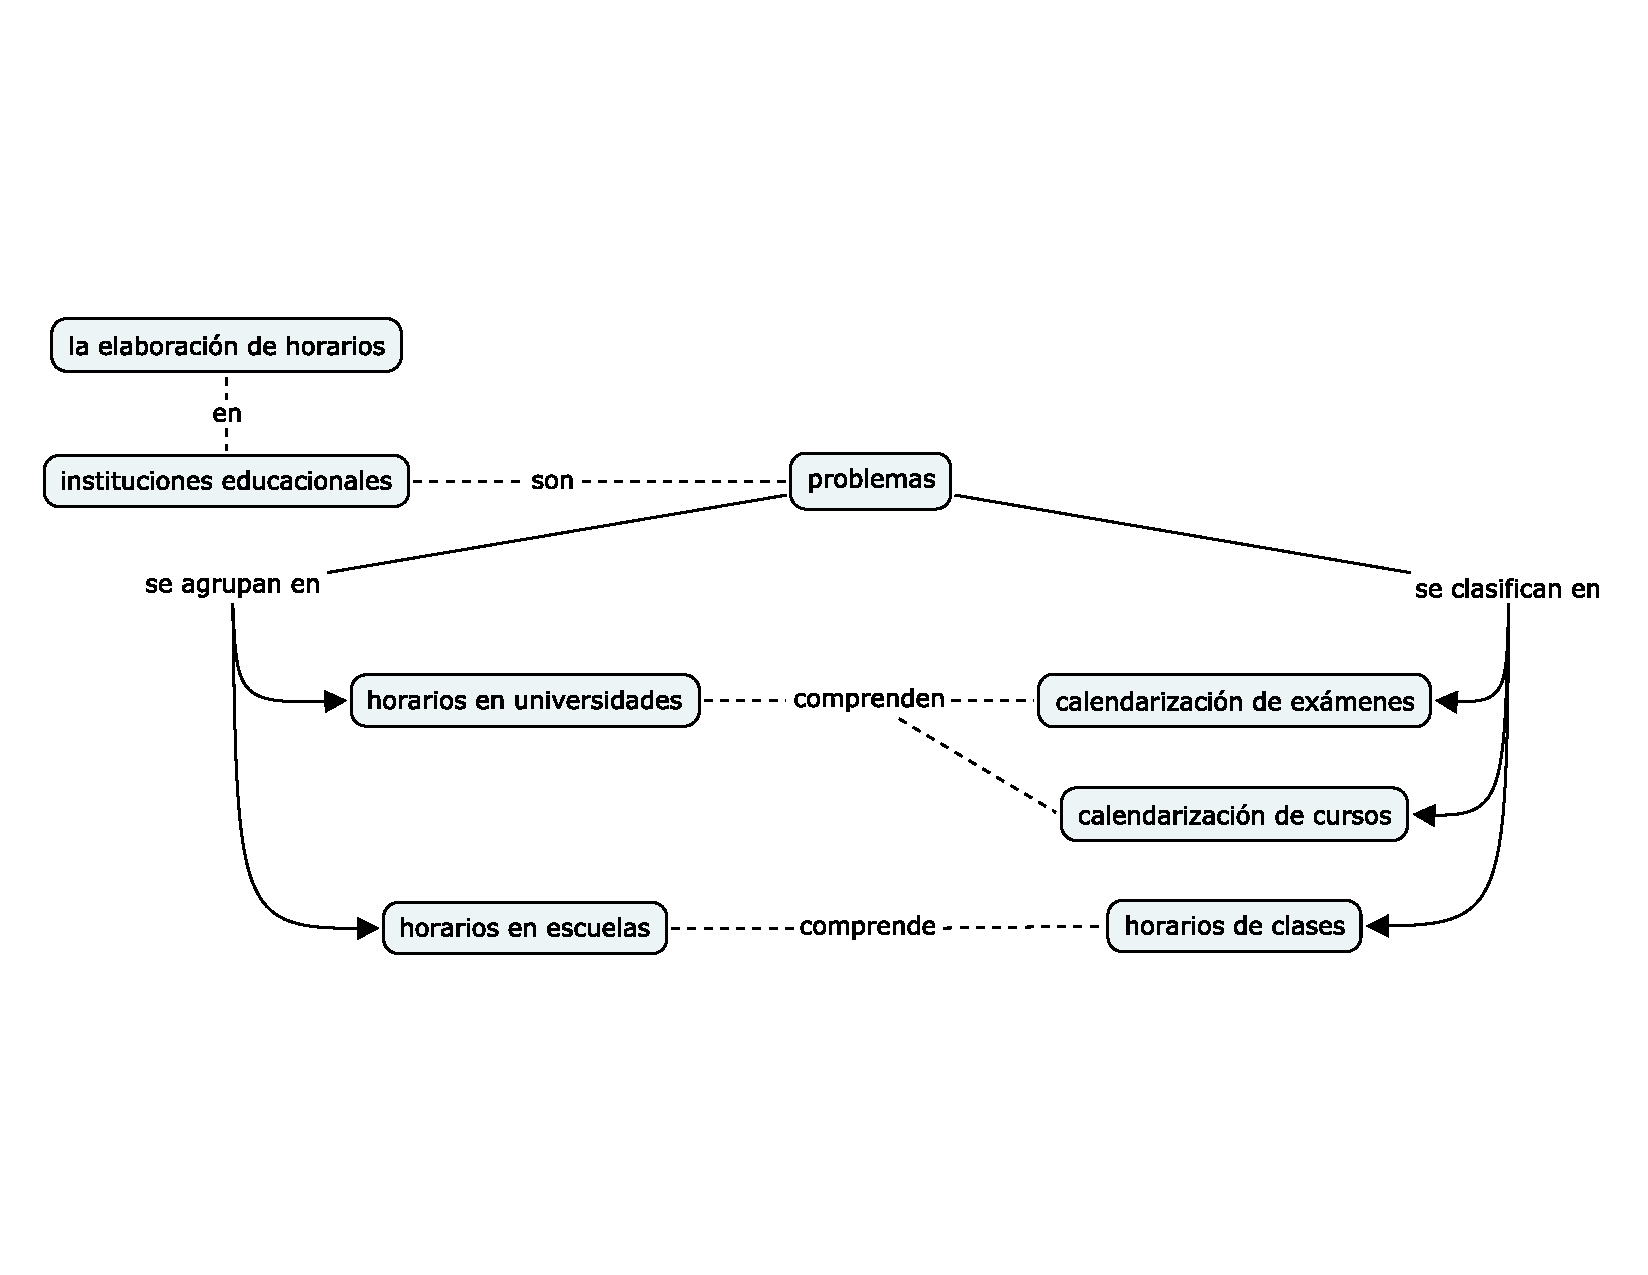
\includegraphics[width=\textwidth]{timetabling_classification.pdf}
\caption[Clasificación del problema]{Clasificación de los problemas en la elaboración de horarios educacionales}
\label{fig:timetabling_classification}
\end{figure}

\subsubsection{Horarios en escuelas}

\index{horarios!en escuelas}

\paragraph{Horarios de clases}

\index{horarios!de clases}
De acuerdo a \citet[p.~88]{schaerf99a-survey-of-automated} el problema de horarios de clases consiste en calendarizar en un periodo semanal todas las clases de una escuela, evitando que los profesores se encuentren con dos clases al mismo tiempo, y viceversa. \citet[p.~10,11]{abdullah06heuristic-approaches} elabora explicando que el problema consiste de un conjunto de profesores, clases, lecciones y periodos semanales. En donde tales periodos semanales son predefinidos.

El problema intenta asignar lecciones a periodos y, un profesor a una clase en particular en un momento dado mientras se satisface un conjunto de restricciones con el fin producir un horario factible. Algunos ejemplos de restricciones en este tipo de problemas son las capacidades de alojamiento, ubicaciones, cargas de trabajo de los profesores, tiempo de descanso entre lecciones.

\subsubsection{Horarios en universidades}

\index{horarios!en universidades}\index{calendarización!de cursos}\index{calendarización!de exámenes}
El problema de la planificación de horarios en universidades puede ser agrupado en dos categorías: (i) calendarización de cursos y (ii) calendarización exámenes.
El problema de la calendarización de cursos es el proceso de la asignación de periodos y aulas de manera tal que las reuniones entre conferenciantes y estudiantes pueda ocurrir.
El problema de la calendarización de exámenes se refiere a la asignación de periodos y aulas de manera tal que los estudiantes puedan presentar sus exámenes.
Ambos problemas son similares de manera superficial, pero existen diferencias importantes que los distinguen.
En la calendarización de exámenes, múltiples exámenes pueden ser presentados en una misma aula (ej. auditorio) al mismo tiempo.
Sin embargo, esto no es posible para la calendarización de cursos en donde únicamente un curso puede ser asignado a un aula \citep[p.~11]{abdullah06heuristic-approaches}.

\paragraph{Calendarización de exámenes}

\index{calendarización!de exámenes}\index{calendarización!de cursos}
\citet[p.~4]{carter95recent-developments} definió el problema como la asignación de exámenes a un número limitado de periodos de manera tal que no existan conflictos o coincidencias. Los problemas de calendarización de cursos y exámenes son similares pero algunas diferencias relevantes según \citet[p.~159]{werra85an-introduction-to-timetabling} son:
\begin{enumerate}[a]
\item Existe generalmente un solo exámen por cada tema (mientras que hay varias exposiciones en un curso)
\item En la calendarización semanal de cursos, el objetivo principal es evitar conflictos (ej. la ocurrencia de que dos cursos elegidos por un mismo estudiante sean programados en el mismo periodo). Para los exámenes, generalmente se pide un máximo de un examen por día para cada estudiante o de ser posible, evitar la calendarización de exámenes en días consecutivos si el periodo de evaluación de exámenes lo permite.
\end{enumerate}
El problema de la calendarización de exámenes es muy común tanto en escuelas como en universidades. La asignación de los exámenes a los periodos está sujeta a un conjunto de limitaciones \citep[p.~12]{abdullah06heuristic-approaches}.

\paragraph{Calendarización de cursos}

\index{calendarización!de cursos}
El problema de la calendarización de cursos surge cuando una universidad (o incluso una escuela) ofrece una colección de cursos (cada uno consistiendo de un número dado de conferencias) sin existir un currículo fijo y en donde cada estudiante puede elegir cierto número de cursos. El problema consiste en la asignación de cada lectura a algún periodo en la semana de manera tal que ningún estudiante requiera asistir a más de una conferencia a la vez \citep[p.~157]{werra85an-introduction-to-timetabling}.
\citet[p.~88]{schaerf99a-survey-of-automated} define el problema como la calendarización semanal de todas las lecciones de un conjunto de cursos universitarios, minimizando los empalmes de las lecciones de cursos teniendo estudiantes en común.
\section*{Diseño de la investigación}
PENDIENTE
\section*{Índice tentativo}
\begin{verbatim}
1. Introducción
1.1. Antecedentes y motivación
1.2. Objetivos de la investigación
1.3. Descripción de la tesis

2. Preliminares
2.1. Introducción
2.2. La programación y sus elementos 
2.2.1. Programa, secuencia, horario
2.2.2. El proceso de programación 
2.2.3. Definiciones
2.3. Historia 
2.3.1. Método de la ruta crítica
2.3.2. Técnica de revisión y evaluación de programas
2.3.3. Desarrollo en otras partes del mundo
2.3.4. El método de diagramación de precedencias
2.3.5. La programación y la computadora

3. Teoría de la programación
3.1. Introducción
3.2. Marco de la programación
3.2.1. Entornos del taller detrabajo
3.2.2. Criterios de evaluación
3.3. Tipología y notación de problemas
3.3.1. Tipología de problemas
3.3.2. Notación
3.4. Áreas de aplicación
3.4.1. Problemas relacionados a laproducción
3.4.2. Otros problemas
3.5. Teoría de la complejidad computacional
3.6. Síntesis de los problemas de programación
3.6.1. Problemas centrales de programación
3.6.2. Problemas enfocados en un recurso único 
3.6.3. Problemas enfocados en múltiples recursos
3.6.4. Problemas de ordenación cíclicos

4. Calendarización en instituciones educacionales 
4.1. Introducción
4.2. Una visión general del problema
4.2.1. El problema general de la programación de horario
4.2.2. Calendarización educacional 
4.2.3. Clasificación de los problemas en el ámbito educacional

5. El gestor escolar

6. Trabajo futuro y conclusiones
6.1. Resumen del trabajo de investigación
6.2. Contribuciones
6.3. Trabajofuturo
6.4. Diseminación 
\end{verbatim}
\section*{Calendario de la investigación}
PENDIENTE
\bibliographystyle{apalike_modified}
\bibliography{/Users/harciga/Dropbox/bibliographies/reviewed,/Users/harciga/Dropbox/bibliographies/Dissertation_books}
\end{document}
